\section{SPI Unit}

The SPI unit provides access to one of the microcontroller's SPI peripherals. It can be configured to use any of the different speeds, clock polarity and phase settings available in its control registers. 

The unit handles up to 16 slave select (NSS) signals and supports message multi-cast (addressing more than one slaves at once). Protection resistors should be used if a multi-cast transaction is issued with MISO connected.

The QUERY command of this unit, illustrated by figure \ref{fig:spi_query}, is flexible enough to support all types of SPI transactions: read-only, write-only, and read-write with different request and response lengths. The slave select pin is held low during the entire transaction.

\begin{figure}[h]
	\centering
	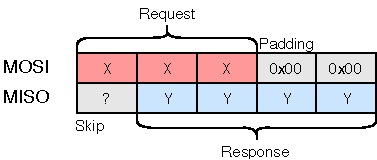
\includegraphics[scale=1.1] {img/spi-query.pdf}
	\caption{\label{fig:spi_query}SPI transaction using the QUERY command}
\end{figure}

\subsection{SPI Configuration}

\begin{inicode}
[SPI:spi@5]
# Peripheral number (SPIx)
device=1
# Pin mappings (SCK,MISO,MOSI)
#  SPI1: (0) A5,A6,A7     (1) B3,B4,B5
#  SPI2: (0) B13,B14,B15
remap=0
# Prescaller: 2,4,8,...,256
prescaller=64
# Clock polarity: 0,1 (clock idle level)
cpol=0
# Clock phase: 0,1 (active edge, 0-first, 1-second)
cpha=0
# Transmit only, disable MISO
tx-only=N
# Bit order (LSB or MSB first)
first-bit=MSB
# SS port name
port=A
# SS pins (comma separated, supports ranges)
pins=0
\end{inicode}

\subsection{SPI Events}

This unit generates no events.

\subsection{SPI Commands}

\begin{tabularx}{\textwidth}{p{\fldwcode}lXp{\fldwpld}}
	\toprule
	\textbf{Code} & \textbf{Name} & \textbf{Function} & \textbf{Payload}  \\	
	\midrule	
	
	0x00 & QUERY & Exchange bytes with a slave device
	& \makecell[tl]{
		\fldreq
		\fld{u8} slave number 0--16 \\
		\fld{u16} response padding \\
		\fld{u16} response length \\
		\fld{u8[]} bytes to write \\
		\fldresp
		\fld{u8[]} received bytes \\		
	} \\
	
	0x01 & MULTICAST & Send a message to multiple slaves at once. The address is a bit map (e.g. 0x8002 = slaves 1 and 15).
	& \makecell[tl]{
		\fldreq
		\fld{u16} addressed slaves \\
		\fld{u8[]} bytes to write
	} \\
	\bottomrule
\end{tabularx}















